\documentclass[12pt,a4paper]{report}
\usepackage[utf8]{inputenc}
\usepackage{amsmath}
\usepackage{amsfonts}
\usepackage{amssymb}
\usepackage{graphicx}
\usepackage{lmodern}

\linespread{2}

\author{Kyle Swanson}
\title{Lab 4: Logic Breadboard}

\begin{document}
\maketitle

\paragraph{}
For this lab, we focused heavily on breadboards. We had a simple launchpad application that would "walk" several IO ports from the binary number 0000 to 1111. The first step was representing this on the breadboard. We used LEDs in a vertical configuration as shown in figure 1. Starting from the right we had bit 0, then 1, and so on. \\
\begin{figure}
	\centering
	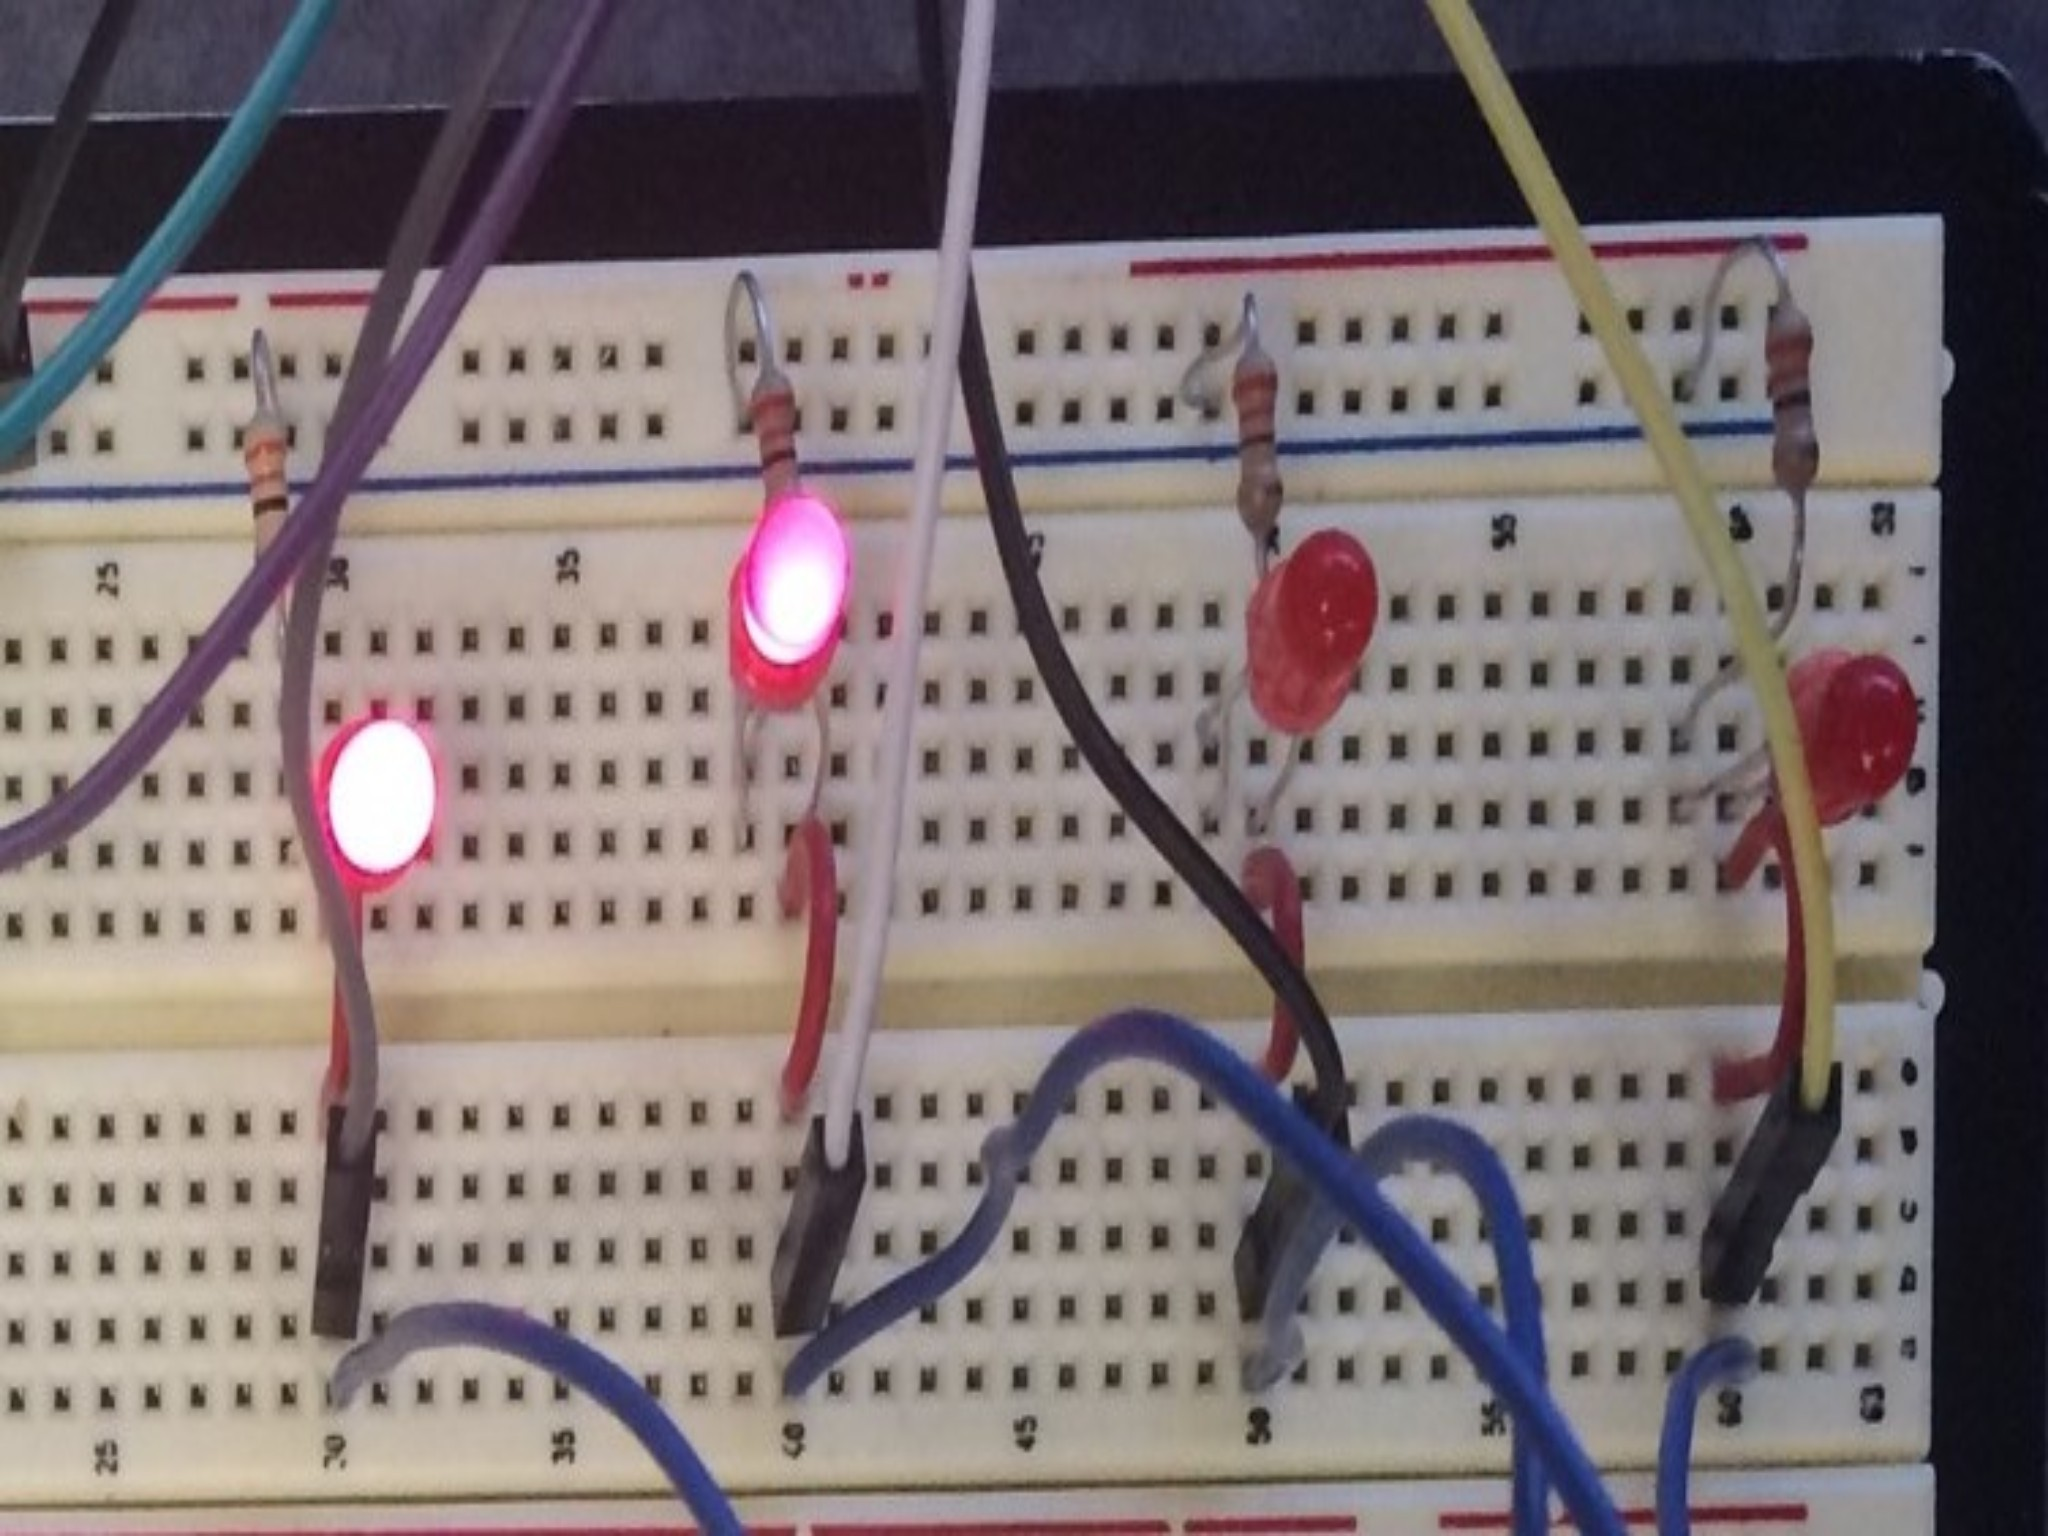
\includegraphics[scale=.1]{img/led_config} \\
	\caption{Our LED Arrangement}
\end{figure}

\end{document}